\chapter{Arquitetura e Modelagem do Sistema} \label{cha:arquitetura}

\section{Arquitetura da Solução}
Esta seção descreve a organização estrutural do sistema ViaBus, que provê funções de gestão de transporte para empresas: cadastro de empresas, usuários, motoristas, veículos, rotas, paradas, viagens e bilhetes. A solução adota uma arquitetura web em camadas, com separação clara entre apresentação (frontend), lógica de negócio e APIs (backend) e persistência (banco de dados).

No \textit{frontend}, utiliza-se Next.js~15 com roteamento via App Router, estado de sessão via NextAuth (estratégia \textit{JWT}) e componentes React tipados (TypeScript). O \textit{frontend} consome APIs REST autenticadas, mantém contexto de usuário/empresa e incorpora mapas e edição geográfica com Leaflet/React-Leaflet para operações sobre rotas e paradas.

O \textit{backend} é implementado com NestJS~11, estruturado por módulos de domínio (\textit{auth}, \textit{users}, \textit{companies}, \textit{drivers}, \textit{vehicles}, \textit{stops}, \textit{routes}, \textit{trips}, \textit{tickets}, etc.). As regras de negócio são expostas por controladores REST, protegidos por autenticação \textit{JWT} e autorização baseada em papéis. A multiempresa é tratada por \textit{companyId} e por um interceptor que injeta o contexto de empresa a partir do token. A persistência usa TypeORM com PostgreSQL.

\begin{figure}[H]
  \centering
  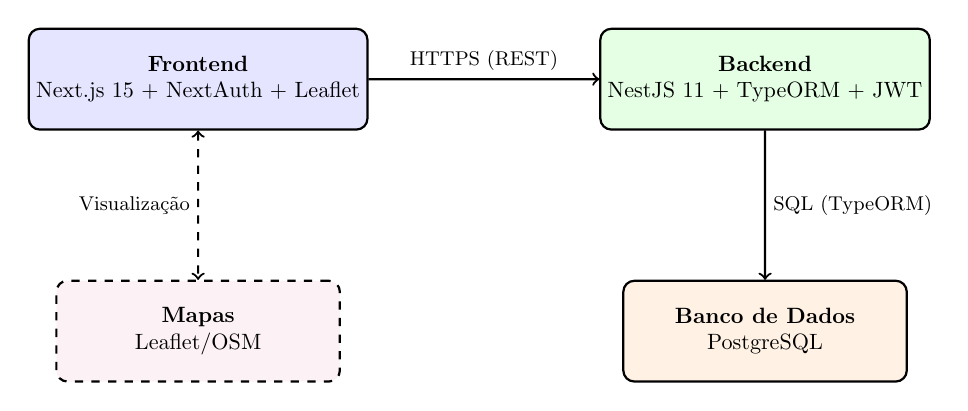
\begin{tikzpicture}[scale=0.8, every node/.style={transform shape}]
    \tikzumlset{font=\footnotesize}
    % Blocos
    \node[draw, rounded corners, thick, fill=blue!10, minimum width=4.5cm, minimum height=1.6cm, align=center] (fe) at (0,2) {\textbf{Frontend}\\Next.js 15 + NextAuth + Leaflet};
    \node[draw, rounded corners, thick, fill=green!10, minimum width=4.5cm, minimum height=1.6cm, align=center] (be) at (9,2) {\textbf{Backend}\\NestJS 11 + TypeORM + JWT};
    \node[draw, rounded corners, thick, fill=orange!10, minimum width=4.5cm, minimum height=1.6cm, align=center] (db) at (9,-2) {\textbf{Banco de Dados}\\PostgreSQL};
    \node[draw, dashed, rounded corners, thick, fill=purple!5, minimum width=4.5cm, minimum height=1.6cm, align=center] (maps) at (0,-2) {\textbf{Mapas}\\Leaflet/OSM};

    % Conexões
    \draw[->, thick] (fe) -- node[above, font=\small]{HTTPS (REST)} (be);
    \draw[->, thick] (be) -- node[right, font=\small]{SQL (TypeORM)} (db);
    \draw[<->, thick, dashed] (fe) -- node[left, font=\small]{Visualização} (maps);
  \end{tikzpicture}
  \caption{Visão de alto nível da solução.}
\end{figure}

\section{Modelagem do Banco de Dados}
O modelo de dados foi projetado para refletir as agregações de negócio. A Tabela~\ref{tab:principais-entidades} sumariza as principais entidades e seus papéis. De forma geral, todas as entidades operacionais são associadas a uma empresa (\textit{multi-tenancy} por chave estrangeira \texttt{company\_id}). Rotas possuem paradas ordenadas (\texttt{route\_stops}) e agenda de operação (\texttt{route\_schedules}); viagens instanciam rotas em horários específicos e originam bilhetes.

\begin{table}[H]
  \centering
  \begin{tabular}{ll}
    \toprule
    \textbf{Entidade}         & \textbf{Descrição resumida}                                               \\
    \midrule
    \texttt{companies}        & Empresa (razão social, nome fantasia, CNPJ, slug, contato)                \\
    \texttt{users}            & Usuário (nome, e-mail, senha, papel, status, \texttt{company\_id})        \\
    \texttt{drivers}          & Motorista (CPF, CNH, categoria, status, \texttt{company\_id})             \\
    \texttt{vehicles}         & Veículo (placa, capacidade, categoria, status, \texttt{company\_id})      \\
    \texttt{addresses}        & Endereço (CEP, logradouro, geocoordenadas)                                \\
    \texttt{stops}            & Parada (nome, \texttt{address\_id}, acessibilidade, \texttt{company\_id}) \\
    \texttt{routes}           & Rota (nome, distância, duração estimada, \texttt{company\_id})            \\
    \texttt{route\_stops}     & Associação rota–parada com ordem e horário opcional                       \\
    \texttt{route\_schedules} & Agenda por dia da semana para a rota                                      \\
    \texttt{trips}            & Viagem (rota, janelas horárias, status, assentos, \texttt{company\_id})   \\
    \texttt{tickets}          & Bilhete (passageiro, preço, assento, pontos de embarque)                  \\
    \bottomrule
  \end{tabular}
  \caption{Principais entidades do domínio.}
  \label{tab:principais-entidades}
\end{table}

O diagrama de classes da Figura~\ref{fig:uml-dominio} sintetiza os relacionamentos mais relevantes do domínio.

\begin{figure}[H]
  \centering
  \begin{tikzpicture}[scale=0.4, every node/.style={transform shape}]
    \tikzumlset{font=\tiny}

    % NÍVEL 1: Empresa (topo da hierarquia)
    \umlclass[x=18,y=25]{Company}{
      id: uuid\\
      legalName: string\\
      tradeName: string\\
      slug: string\\
      cnpj: string\\
      email: string\\
      phone: string\\
      logoUrl: string\\
      createdAt: Date\\
      updatedAt: Date
    }{ }

    % NÍVEL 2: Gestão de usuários e recursos
    \umlclass[x=3,y=18]{User}{
      id: uuid\\
      name: string\\
      email: string\\
      phone: string\\
      photoUrl: string\\
      password: string\\
      role: UserRole\\
      status: UserStatus\\
      companyId: uuid\\
      createdAt: Date\\
      updatedAt: Date
    }{ }

    \umlclass[x=18,y=18]{Vehicle}{
      id: uuid\\
      plate: string\\
      model: string\\
      brand: string\\
      year: number\\
      capacity: number\\
      category: VehicleCategory\\
      comfortConfiguration: ComfortConfiguration\\
      busType: BusType\\
      acquisitionDate: Date\\
      odometer: number\\
      lastMaintenance: Date\\
      nextMaintenance: Date\\
      status: VehicleStatus\\
      notes: string\\
      companyId: uuid
    }{ }

    \umlclass[x=33,y=18]{Driver}{
      id: uuid\\
      name: string\\
      cpf: string\\
      licenseNumber: string\\
      licenseCategory: string\\
      licenseExpiry: Date\\
      phone: string\\
      email: string\\
      birthDate: Date\\
      hireDate: Date\\
      status: DriverStatus\\
      emergencyContactName: string\\
      emergencyContactPhone: string\\
      address: string\\
      notes: string\\
      companyId: uuid
    }{ }

    % NÍVEL 3: Configuração de rotas
    \umlclass[x=8,y=11]{Route}{
      id: uuid\\
      name: string\\
      description: string\\
      isActive: boolean\\
      estimatedDuration: string\\
      distance: number\\
      companyId: uuid
    }{ }

    \umlclass[x=23,y=11]{Stop}{
      id: uuid\\
      name: string\\
      addressId: uuid\\
      isActive: boolean\\
      hasAccessibility: boolean\\
      hasShelter: boolean\\
      companyId: uuid
    }{ }

    \umlclass[x=38,y=11]{Address}{
      id: uuid\\
      cep: string\\
      street: string\\
      number: string\\
      complement: string\\
      neighborhood: string\\
      city: string\\
      state: string\\
      longitude: number\\
      latitude: number\\
      createdAt: Date\\
      updatedAt: Date
    }{ }

    % NÍVEL 4: Relacionamentos de configuração
    \umlclass[x=8,y=4]{RouteSchedule}{
      id: uuid\\
      routeId: uuid\\
      dayOfWeek: number\\
      isActive: boolean\\
      createdAt: Date\\
      updatedAt: Date
    }{ }

    \umlclass[x=23,y=4]{RouteStop}{
      id: uuid\\
      routeId: uuid\\
      stopId: uuid\\
      order: number\\
      departureTime: string
    }{ }

    % NÍVEL 5: Operação - Viagens
    \umlclass[x=3,y=-3]{TripVehicle}{
      id: uuid\\
      tripId: uuid\\
      vehicleId: uuid\\
      primaryDriverId: uuid\\
      secondaryDriverId: uuid\\
      isActive: boolean\\
      observations: string\\
      createdAt: Date\\
      updatedAt: Date
    }{ }

    \umlclass[x=18,y=-3]{Trip}{
      id: uuid\\
      routeId: uuid\\
      departureTime: Date\\
      estimatedArrivalTime: Date\\
      actualDepartureTime: Date\\
      actualArrivalTime: Date\\
      status: TripStatus\\
      basePrice: number\\
      totalSeats: number\\
      availableSeats: number\\
      isAutoGenerated: boolean\\
      observations: string\\
      companyId: uuid\\
      createdAt: Date\\
      updatedAt: Date
    }{ }

    % NÍVEL 6: Vendas - Bilhetes
    \umlclass[x=33,y=-3]{Ticket}{
      id: uuid\\
      tripId: uuid\\
      passengerName: string\\
      passengerDocument: string\\
      passengerPhone: string\\
      passengerEmail: string\\
      seatNumber: string\\
      price: number\\
      status: TicketStatus\\
      boardingPointType: BoardingPointType\\
      boardingStopId: uuid\\
      boardingLocationDescription: string\\
      boardingLatitude: number\\
      boardingLongitude: number\\
      landingPointType: BoardingPointType\\
      landingStopId: uuid\\
      landingLocationDescription: string\\
      landingLatitude: number\\
      landingLongitude: number\\
      observations: string\\
      companyId: uuid
    }{ }

    % RELACIONAMENTOS HIERÁRQUICOS PRINCIPAIS
    % Company -> Recursos
    \umlassoc[mult1=1,mult2=*]{Company}{User}
    \umlassoc[mult1=1,mult2=*]{Company}{Vehicle}
    \umlassoc[mult1=1,mult2=*]{Company}{Driver}

    % Company -> Configuração
    \umlassoc[mult1=1,mult2=*,arm1=-135,arm2=90]{Company}{Route}
    \umlassoc[mult1=1,mult2=*,arm1=-45,arm2=90]{Company}{Stop}

    % Configuração de endereços
    \umlassoc[mult1=1,mult2=*]{Address}{Stop}

    % FLUXO PRINCIPAL: Route -> RouteStop <- Stop
    \umlassoc[mult1=1,mult2=*]{Route}{RouteStop}
    \umlassoc[mult1=1,mult2=*]{Stop}{RouteStop}

    % Horários das rotas
    \umlassoc[mult1=1,mult2=*]{Route}{RouteSchedule}

    % FLUXO OPERACIONAL: Route -> Trip
    \umlassoc[mult1=1,mult2=*]{Route}{Trip}
    \umlassoc[mult1=1,mult2=*,arm1=-135,arm2=90]{Company}{Trip}

    % Trip -> TripVehicle (associação veículo/motorista)
    \umlassoc[mult1=1,mult2=*]{Trip}{TripVehicle}
    \umlassoc[mult1=1,mult2=*,arm1=-90,arm2=90]{Vehicle}{TripVehicle}
    \umlassoc[mult1=1,mult2=*,arm1=-90,arm2=135,stereo=<<primaryDriver>>]{Driver}{TripVehicle}

    % FLUXO DE VENDAS: Trip -> Ticket
    \umlassoc[mult1=1,mult2=*]{Trip}{Ticket}
    \umlassoc[mult1=1,mult2=*,arm1=-45,arm2=135]{Company}{Ticket}

    % Relacionamento opcional: Stop -> Ticket (embarque/desembarque específico)
    \umldep[stereo=<<boarding/landing>>,mult1=0..1,mult2=*,arm1=-90,arm2=135]{Stop}{Ticket}

  \end{tikzpicture}
  \caption{Diagrama de classes detalhado do domínio ViaBus.}
  \label{fig:uml-dominio}
\end{figure}

\subsection{Diagramas UML Fracionados por Agregado}
Para facilitar a leitura, os diagramas a seguir detalham os principais agregados do domínio.

\subsubsection*{Agregado Organizacional: Empresas e Usuários}
\begin{figure}[H]
  \centering
  \begin{tikzpicture}[scale=0.8, every node/.style={transform shape}]
    \tikzumlset{font=\tiny}
    \umlclass[x=0,y=0]{Company}{
      id: uuid\\
      legalName: string\\
      tradeName: string\\
      slug: string\\
      cnpj: string\\
      email: string\\
      phone: string\\
      logoUrl: string\\
      createdAt: Date\\
      updatedAt: Date
    }{ }
    \umlclass[x=8,y=0]{User}{
      id: uuid\\
      name: string\\
      email: string\\
      phone: string\\
      photoUrl: string\\
      password: string\\
      role: UserRole\\
      status: UserStatus\\
      companyId: uuid\\
      createdAt: Date\\
      updatedAt: Date
    }{ }
    \umlassoc[mult1=1,mult2=*]{Company}{User}
    \umlnote[x=0,y=-4, width=12cm]{Company}{Escopo multiempresa: todas as entidades operacionais possuem \texttt{companyId} para isolamento de dados}
  \end{tikzpicture}
  \caption{Agregado organizacional - estrutura multiempresa.}
\end{figure}

\subsubsection*{Agregado de Rotas e Paradas}
\begin{figure}[H]
  \centering
  \begin{tikzpicture}[scale=0.7, every node/.style={transform shape}]
    \tikzumlset{font=\tiny}
    \umlclass[x=0,y=2]{Address}{
      id: uuid\\
      cep: string\\
      street: string\\
      number: string\\
      complement: string\\
      neighborhood: string\\
      city: string\\
      state: string\\
      latitude: number\\
      longitude: number\\
      createdAt: Date\\
      updatedAt: Date
    }{ }
    \umlclass[x=8,y=2]{Stop}{
      id: uuid\\
      name: string\\
      addressId: uuid\\
      isActive: boolean\\
      hasAccessibility: boolean\\
      hasShelter: boolean\\
      companyId: uuid
    }{ }
    \umlclass[x=0,y=-3]{RouteSchedule}{
      id: uuid\\
      routeId: uuid\\
      dayOfWeek: number\\
      isActive: boolean\\
      createdAt: Date\\
      updatedAt: Date
    }{ }
    \umlclass[x=6,y=-3]{Route}{
      id: uuid\\
      name: string\\
      description: string\\
      isActive: boolean\\
      estimatedDuration: string\\
      distance: number\\
      companyId: uuid
    }{ }
    \umlclass[x=12,y=-3]{RouteStop}{
      id: uuid\\
      routeId: uuid\\
      stopId: uuid\\
      order: number\\
      departureTime: string
    }{ }
    \umlassoc[mult1=1,mult2=*]{Address}{Stop}
    \umlassoc[mult1=1,mult2=*]{Route}{RouteStop}
    \umlassoc[mult1=1,mult2=*]{Stop}{RouteStop}
    \umlassoc[mult1=1,mult2=*]{Route}{RouteSchedule}
    \umlnote[x=4,y=-6, width=10cm]{Route}{RouteStop implementa relacionamento many-to-many entre Route e Stop com ordem e horários específicos}
  \end{tikzpicture}
  \caption{Agregado de configuração de rotas, paradas e horários.}
\end{figure}

\subsubsection*{Agregado de Recursos Operacionais}
\begin{figure}[H]
  \centering
  \begin{tikzpicture}[scale=0.7, every node/.style={transform shape}]
    \tikzumlset{font=\tiny}
    \umlclass[x=0,y=2]{Vehicle}{
      id: uuid\\
      plate: string\\
      model: string\\
      brand: string\\
      year: number\\
      capacity: number\\
      category: VehicleCategory\\
      comfortConfiguration: ComfortConfiguration\\
      busType: BusType\\
      acquisitionDate: Date\\
      odometer: number\\
      lastMaintenance: Date\\
      nextMaintenance: Date\\
      status: VehicleStatus\\
      notes: string\\
      companyId: uuid
    }{ }
    \umlclass[x=15,y=2]{Driver}{
      id: uuid\\
      name: string\\
      cpf: string\\
      licenseNumber: string\\
      licenseCategory: string\\
      licenseExpiry: Date\\
      phone: string\\
      email: string\\
      birthDate: Date\\
      hireDate: Date\\
      status: DriverStatus\\
      emergencyContactName: string\\
      emergencyContactPhone: string\\
      address: string\\
      notes: string\\
      companyId: uuid
    }{ }
    \umlclass[x=7.5,y=-2]{TripVehicle}{
      id: uuid\\
      tripId: uuid\\
      vehicleId: uuid\\
      primaryDriverId: uuid\\
      secondaryDriverId: uuid\\
      isActive: boolean\\
      observations: string\\
      createdAt: Date\\
      updatedAt: Date
    }{ }
    \umlassoc[mult1=1,mult2=*]{Vehicle}{TripVehicle}
    \umlassoc[mult1=1,mult2=*,stereo=<<primaryDriver>>]{Driver}{TripVehicle}
    \umlnote[x=2,y=-6, width=16cm]{TripVehicle}{TripVehicle associa dinamicamente veículos e motoristas às viagens. Um veículo pode ter motorista principal e secundário por viagem}
  \end{tikzpicture}
  \caption{Agregado de recursos operacionais - frota e motoristas.}
\end{figure}

\subsubsection*{Agregado de Operação e Vendas}
\begin{figure}[H]
  \centering
  \begin{tikzpicture}[scale=0.6, every node/.style={transform shape}]
    \tikzumlset{font=\tiny}
    \umlclass[x=6,y=3]{Trip}{
      id: uuid\\
      routeId: uuid\\
      departureTime: Date\\
      estimatedArrivalTime: Date\\
      actualDepartureTime: Date\\
      actualArrivalTime: Date\\
      status: TripStatus\\
      basePrice: number\\
      totalSeats: number\\
      availableSeats: number\\
      isAutoGenerated: boolean\\
      observations: string\\
      companyId: uuid\\
      createdAt: Date\\
      updatedAt: Date
    }{ }
    \umlclass[x=0,y=0]{TripVehicle}{
      id: uuid\\
      tripId: uuid\\
      vehicleId: uuid\\
      primaryDriverId: uuid\\
      secondaryDriverId: uuid\\
      isActive: boolean\\
      observations: string\\
      createdAt: Date\\
      updatedAt: Date
    }{ }
    \umlclass[x=12,y=0]{Ticket}{
      id: uuid\\
      tripId: uuid\\
      passengerName: string\\
      passengerDocument: string\\
      passengerPhone: string\\
      passengerEmail: string\\
      seatNumber: string\\
      price: number\\
      status: TicketStatus\\
      boardingPointType: BoardingPointType\\
      boardingStopId: uuid\\
      boardingLocationDescription: string\\
      landingPointType: BoardingPointType\\
      landingStopId: uuid\\
      landingLocationDescription: string\\
      observations: string\\
      companyId: uuid
    }{ }
    \umlclass[x=18,y=3]{Stop}{
      id: uuid\\
      name: string\\
      companyId: uuid
    }{ }
    \umlassoc[mult1=1,mult2=*]{Trip}{TripVehicle}
    \umlassoc[mult1=1,mult2=*]{Trip}{Ticket}
    \umldep[stereo=<<boarding/landing>>,mult1=0..1,mult2=*]{Stop}{Ticket}
    \umlnote[x=1,y=-4, width=14cm]{Trip}{TripVehicle associa veículos e motoristas às viagens. Ticket permite embarque/desembarque em paradas específicas ou localizações customizadas}
  \end{tikzpicture}
  \caption{Agregado de operação - viagens, recursos e vendas.}
\end{figure}

\section{Arquitetura do Backend}

O backend implementa uma arquitetura modular baseada no framework NestJS 11, seguindo os princípios de \textit{Separation of Concerns} e \textit{Dependency Injection}. A aplicação é estruturada em 10 módulos de domínio, com camadas bem definidas de segurança, validação e persistência.

\subsection{Organização Modular}

O sistema está organizado em três grupos funcionais de módulos, conforme ilustrado na Figura~\ref{fig:backend-modules}.

\begin{figure}[H]
  \centering
  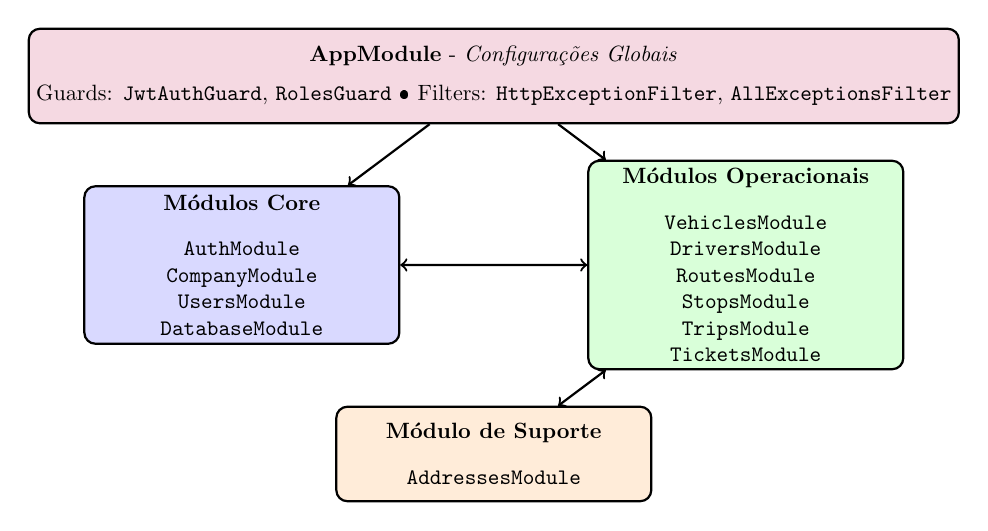
\begin{tikzpicture}[scale=0.8, every node/.style={transform shape}]
    % Módulos Core
    \node[draw, rounded corners, thick, fill=blue!15, minimum width=5cm, minimum height=2.5cm, align=center] (core) at (0,3) {
      \textbf{Módulos Core}\\[0.3cm]
      \texttt{AuthModule}\\
      \texttt{CompanyModule}\\
      \texttt{UsersModule}\\
      \texttt{DatabaseModule}
    };

    % Módulos Operacionais
    \node[draw, rounded corners, thick, fill=green!15, minimum width=5cm, minimum height=3cm, align=center] (operational) at (8,3) {
      \textbf{Módulos Operacionais}\\[0.3cm]
      \texttt{VehiclesModule}\\
      \texttt{DriversModule}\\
      \texttt{RoutesModule}\\
      \texttt{StopsModule}\\
      \texttt{TripsModule}\\
      \texttt{TicketsModule}
    };

    % Módulos de Suporte
    \node[draw, rounded corners, thick, fill=orange!15, minimum width=5cm, minimum height=1.5cm, align=center] (support) at (4,0) {
      \textbf{Módulo de Suporte}\\[0.3cm]
      \texttt{AddressesModule}
    };

    % AppModule
    \node[draw, rounded corners, thick, fill=purple!15, minimum width=10cm, minimum height=1.5cm, align=center] (app) at (4,6) {
      \textbf{AppModule} - \textit{Configurações Globais}\\[0.2cm]
      Guards: \texttt{JwtAuthGuard}, \texttt{RolesGuard} • Filters: \texttt{HttpExceptionFilter}, \texttt{AllExceptionsFilter}
    };

    % Setas
    \draw[->, thick] (app) -- (core);
    \draw[->, thick] (app) -- (operational);
    \draw[<->, thick] (core) -- (operational);
    \draw[<->, thick] (support) -- (operational);
  \end{tikzpicture}
  \caption{Organização modular do backend ViaBus.}
  \label{fig:backend-modules}
\end{figure}

A organização modular agrupa os componentes por responsabilidade funcional. Os \textbf{Módulos Core} gerenciam autenticação, usuários, empresas e configuração de banco de dados. Os \textbf{Módulos Operacionais} implementam as regras de negócio específicas do domínio de transporte. O \textbf{Módulo de Suporte} fornece funcionalidades auxiliares como geocodificação. O \texttt{AppModule} centraliza as configurações globais de segurança e tratamento de erros, aplicadas a todos os módulos.

\subsection{Pipeline de Processamento}

Cada requisição HTTP passa por um pipeline estruturado de middleware, guards, interceptors e filters, garantindo segurança e consistência.

\begin{figure}[H]
  \centering
  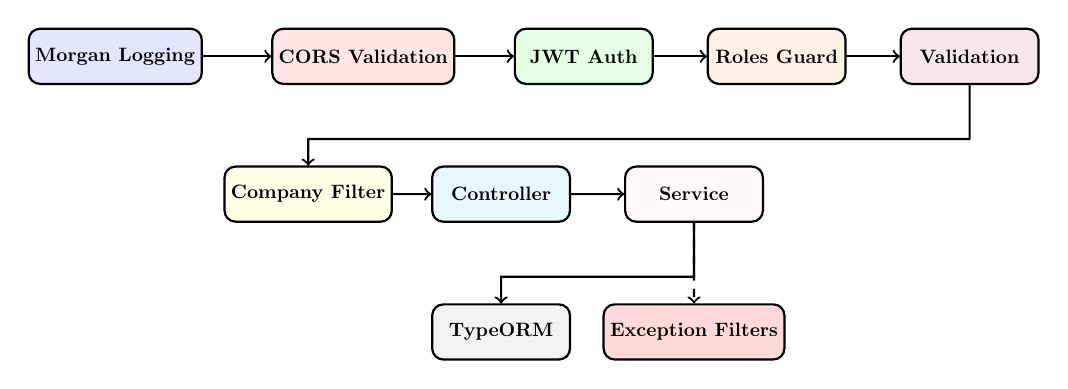
\begin{tikzpicture}[scale=0.7, every node/.style={transform shape}]
    % Pipeline stages
    \node[draw, rounded corners, thick, fill=blue!10, minimum width=2.5cm, minimum height=1cm] (morgan) at (0,0) {\textbf{Morgan Logging}};
    \node[draw, rounded corners, thick, fill=red!10, minimum width=2.5cm, minimum height=1cm] (cors) at (4.5,0) {\textbf{CORS Validation}};
    \node[draw, rounded corners, thick, fill=green!10, minimum width=2.5cm, minimum height=1cm] (jwt) at (8.5,0) {\textbf{JWT Auth}};
    \node[draw, rounded corners, thick, fill=orange!10, minimum width=2.5cm, minimum height=1cm] (roles) at (12,0) {\textbf{Roles Guard}};
    \node[draw, rounded corners, thick, fill=purple!10, minimum width=2.5cm, minimum height=1cm] (validation) at (15.5,0) {\textbf{Validation}};

    \node[draw, rounded corners, thick, fill=yellow!10, minimum width=3cm, minimum height=1cm] (interceptor) at (3.5,-2.5) {\textbf{Company Filter}};
    \node[draw, rounded corners, thick, fill=cyan!10, minimum width=2.5cm, minimum height=1cm] (controller) at (7,-2.5) {\textbf{Controller}};
    \node[draw, rounded corners, thick, fill=pink!10, minimum width=2.5cm, minimum height=1cm] (service) at (10.5,-2.5) {\textbf{Service}};

    \node[draw, rounded corners, thick, fill=gray!10, minimum width=2.5cm, minimum height=1cm] (typeorm) at (7,-5) {\textbf{TypeORM}};
    \node[draw, rounded corners, thick, fill=red!15, minimum width=3cm, minimum height=1cm] (filters) at (10.5,-5) {\textbf{Exception Filters}};

    % Arrows
    \draw[->, thick] (morgan) -- (cors);
    \draw[->, thick] (cors) -- (jwt);
    \draw[->, thick] (jwt) -- (roles);
    \draw[->, thick] (roles) -- (validation);
    \draw[->, thick] (validation) -- ++(0,-1.5) -| (interceptor);
    \draw[->, thick] (interceptor) -- (controller);
    \draw[->, thick] (controller) -- (service);
    \draw[->, thick] (service) -- ++(0,-1.5) -| (typeorm);
    \draw[->, thick, dashed] (service) -- (filters);
  \end{tikzpicture}
  \caption{Pipeline de processamento de requisições.}
  \label{fig:request-pipeline}
\end{figure}

O pipeline garante que cada requisição passe por validações sequenciais obrigatórias. Inicialmente, o \textbf{Morgan} registra logs e o \textbf{CORS} valida origens permitidas. A autenticação via \textbf{JwtAuthGuard} verifica tokens válidos, seguida da autorização por \textbf{RolesGuard} que confirma permissões do usuário. O \textbf{ValidationPipe} valida DTOs de entrada. O \textbf{CompanyFilterInterceptor} injeta o contexto multiempresa antes do processamento pelo \textbf{Controller} e \textbf{Service}. Finalmente, o \textbf{TypeORM} persiste dados e os \textbf{Exception Filters} tratam erros de forma padronizada.

\subsection{Fluxo de Autenticação}

O sistema utiliza autenticação baseada em JWT com suporte a multi-tenancy. A Figura~\ref{fig:auth-sequence} detalha o processo completo.

\begin{figure}[H]
  \centering
  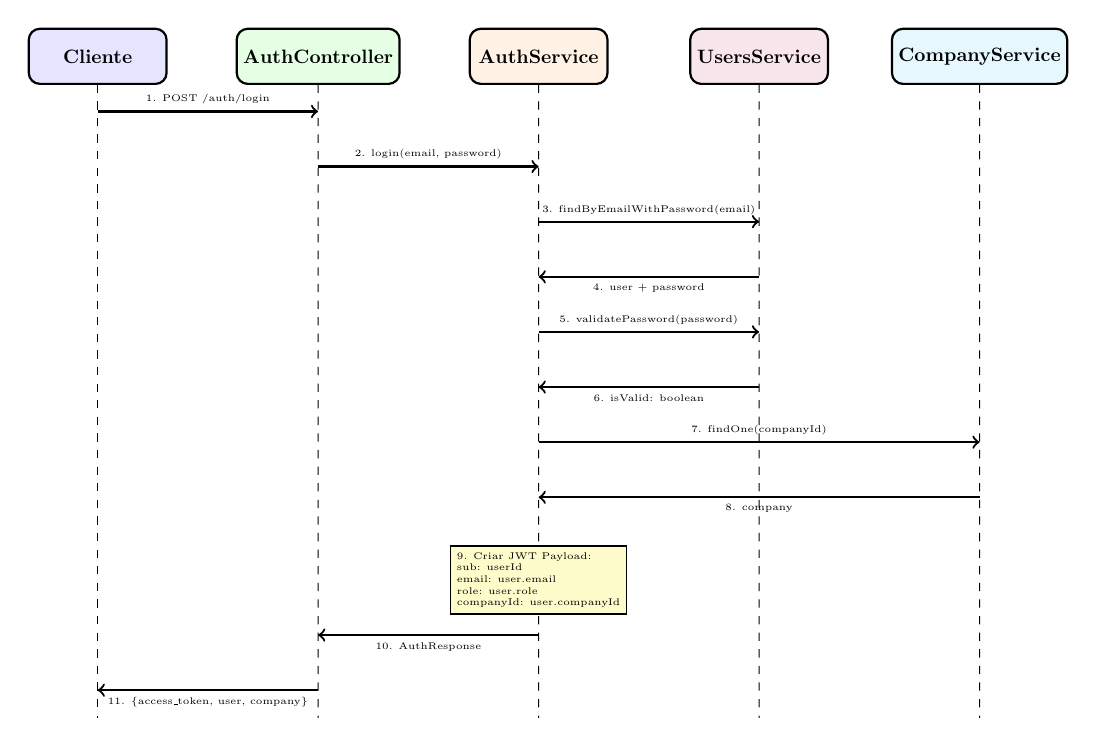
\begin{tikzpicture}[scale=0.7, every node/.style={transform shape}]
    % Participantes
    \node[draw, rounded corners, thick, fill=blue!10, minimum width=2.5cm, minimum height=1cm] (client) at (0,11) {\textbf{Cliente}};
    \node[draw, rounded corners, thick, fill=green!10, minimum width=2.5cm, minimum height=1cm] (auth) at (4,11) {\textbf{AuthController}};
    \node[draw, rounded corners, thick, fill=orange!10, minimum width=2.5cm, minimum height=1cm] (service) at (8,11) {\textbf{AuthService}};
    \node[draw, rounded corners, thick, fill=purple!10, minimum width=2.5cm, minimum height=1cm] (users) at (12,11) {\textbf{UsersService}};
    \node[draw, rounded corners, thick, fill=cyan!10, minimum width=2.5cm, minimum height=1cm] (company) at (16,11) {\textbf{CompanyService}};

    % Linhas de vida
    \draw[dashed] (client) -- (0,-1);
    \draw[dashed] (auth) -- (4,-1);
    \draw[dashed] (service) -- (8,-1);
    \draw[dashed] (users) -- (12,-1);
    \draw[dashed] (company) -- (16,-1);

    % Mensagens
    \draw[->, thick] (0,10) -- node[above, font=\tiny]{1. POST /auth/login} (4,10);
    \draw[->, thick] (4,9) -- node[above, font=\tiny]{2. login(email, password)} (8,9);
    \draw[->, thick] (8,8) -- node[above, font=\tiny]{3. findByEmailWithPassword(email)} (12,8);
    \draw[<-, thick] (8,7) -- node[below, font=\tiny]{4. user + password} (12,7);
    \draw[->, thick] (8,6) -- node[above, font=\tiny]{5. validatePassword(password)} (12,6);
    \draw[<-, thick] (8,5) -- node[below, font=\tiny]{6. isValid: boolean} (12,5);
    \draw[->, thick] (8,4) -- node[above, font=\tiny]{7. findOne(companyId)} (16,4);
    \draw[<-, thick] (8,3) -- node[below, font=\tiny]{8. company} (16,3);

    % Processamento interno
    \node[draw, fill=yellow!20, align=left, font=\tiny] at (8,1.5) {9. Criar JWT Payload:\\sub: userId\\email: user.email\\role: user.role\\companyId: user.companyId};

    \draw[<-, thick] (4,0.5) -- node[below, font=\tiny]{10. AuthResponse} (8,0.5);
    \draw[<-, thick] (0,-0.5) -- node[below, font=\tiny]{11. \{access\_token, user, company\}} (4,-0.5);
  \end{tikzpicture}
  \caption{Diagrama de sequência - fluxo de autenticação.}
  \label{fig:auth-sequence}
\end{figure}

O fluxo de autenticação implementa um processo seguro e eficiente em 11 etapas. O cliente envia credenciais via POST para o \texttt{AuthController}, que delega ao \texttt{AuthService} a validação. O \texttt{UsersService} busca o usuário por email (incluindo senha hash), valida a senha fornecida e retorna o resultado. Confirmada a autenticação, o \texttt{AuthService} consulta os dados da empresa via \texttt{CompanyService} e cria o payload JWT contendo informações do usuário e contexto empresarial. A resposta final inclui o token de acesso, dados do usuário e informações da empresa, permitindo que o frontend mantenha o contexto de sessão multiempresa.

\subsection{Arquitetura Multi-tenant}

O sistema implementa isolamento de dados por empresa através de uma arquitetura multi-tenant baseada em filtros automáticos. A solução utiliza três componentes principais que trabalham em conjunto para garantir separação completa entre inquilinos:

\begin{itemize}
  \item \textbf{BaseCompanyService<T>}: Classe abstrata que implementa operações CRUD com filtro automático por \texttt{companyId}
  \item \textbf{CompanyFilterInterceptor}: Interceptor que extrai o \texttt{companyId} do token JWT e o injeta no contexto da requisição
  \item \textbf{@CurrentUser}: Decorator que facilita o acesso aos dados do usuário autenticado
\end{itemize}

A implementação garante que todas as operações de banco de dados incluam automaticamente a cláusula \texttt{WHERE companyId = ?}, eliminando a possibilidade de vazamento de dados entre empresas. O padrão é aplicado consistentemente em todos os módulos operacionais (usuários, motoristas, veículos, rotas, paradas, viagens e passagens).

\begin{figure}[H]
  \centering
  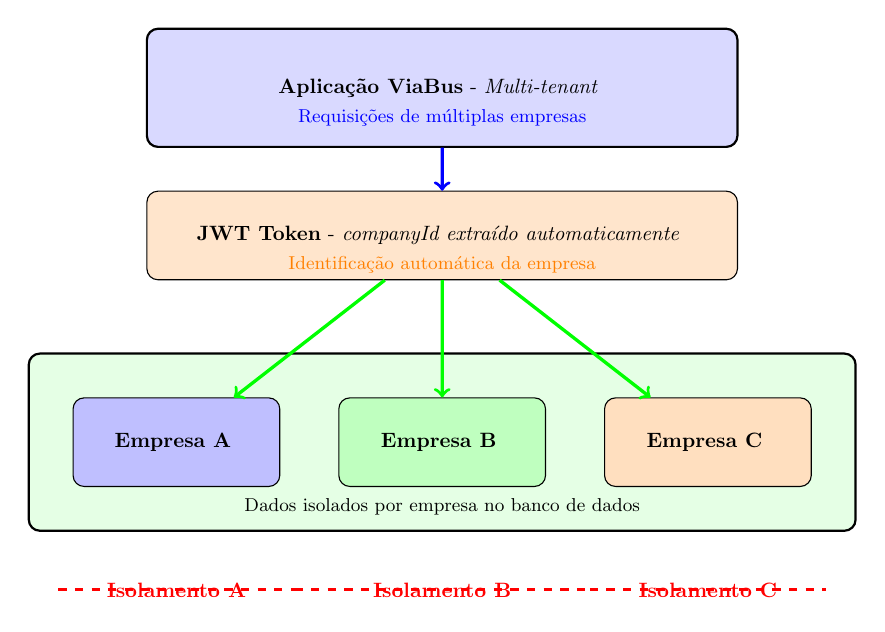
\begin{tikzpicture}[scale=0.75, every node/.style={transform shape}]
    % Single application instance
    \node[draw, rounded corners, thick, fill=blue!15, minimum width=10cm, minimum height=2cm, align=center] (app) at (7,8) {
      \textbf{Aplicação ViaBus} - \textit{Multi-tenant}
    };

    % JWT Token extraction with better positioning
    \node[draw, rounded corners, fill=orange!20, minimum width=10cm, minimum height=1.5cm, align=center] (jwt) at (7,5.5) {
      \textbf{JWT Token} - \textit{companyId extraído automaticamente}
    };

    % Database container - background
    \node[draw, rounded corners, thick, fill=green!10, minimum width=14cm, minimum height=3cm, align=center] (dbContainer) at (7,2) {

    };

    % Tenant A data - positioned above background
    \node[draw, rounded corners, fill=blue!25, minimum width=3.5cm, minimum height=1.5cm, align=center] (tenantA) at (2.5,2) {
      \textbf{Empresa A}
    };

    % Tenant B data - positioned above background
    \node[draw, rounded corners, fill=green!25, minimum width=3.5cm, minimum height=1.5cm, align=center] (tenantB) at (7,2) {
      \textbf{Empresa B}
    };

    % Tenant C data - positioned above background
    \node[draw, rounded corners, fill=orange!25, minimum width=3.5cm, minimum height=1.5cm, align=center] (tenantC) at (11.5,2) {
      \textbf{Empresa C}
    };

    % Flow arrows with better positioning
    \draw[->, very thick, blue] (app) -- (jwt);
    \draw[->, very thick, green] (jwt) -- (tenantA);
    \draw[->, very thick, green] (jwt) -- (tenantB);
    \draw[->, very thick, green] (jwt) -- (tenantC);

    % Isolation lines - positioned below the tenant boxes
    \draw[dashed, very thick, red] (0.5,-0.5) -- (4.5,-0.5);
    \draw[dashed, very thick, red] (4.5,-0.5) -- (9.5,-0.5);
    \draw[dashed, very thick, red] (9.5,-0.5) -- (13.5,-0.5);

    % Isolation labels - positioned below the lines
    \node[text=red, font=\small, font=\bfseries] at (2.5,-0.5) {Isolamento A};
    \node[text=red, font=\small, font=\bfseries] at (7,-0.5) {Isolamento B};
    \node[text=red, font=\small, font=\bfseries] at (11.5,-0.5) {Isolamento C};

    % Data flow explanation
    \node[text=blue, font=\small, align=center] at (7,7.5) {Requisições de múltiplas empresas};
    \node[text=orange, font=\small, align=center] at (7,5) {Identificação automática da empresa};
    \node[text=black, font=\small, align=center] at (7,0.9) {Dados isolados por empresa no banco de dados};
  \end{tikzpicture}
  \caption{Arquitetura multi-tenant: uma aplicação serve múltiplas empresas com isolamento automático de dados.}
  \label{fig:multi-tenant-simple}
\end{figure}

\section{Arquitetura do Frontend}

O frontend implementa uma arquitetura moderna baseada em Next.js~15 (React~19) com App Router, utilizando TypeScript para tipagem estática completa. A aplicação segue padrões de arquitetura limpa e organização por domínio.

\subsection{Stack Tecnológico e Organização}

O frontend utiliza um conjunto integrado de tecnologias modernas para garantir performance, experiência do usuário e manutenibilidade:

\begin{itemize}
  \item \textbf{Framework}: Next.js~15 com App Router para roteamento baseado em arquivo
  \item \textbf{UI}: React~19 com componentes Radix UI e estilização Tailwind CSS
  \item \textbf{Formulários}: React Hook Form + Zod para validação tipada
  \item \textbf{Autenticação}: NextAuth v4 com JWT e provedores customizados
  \item \textbf{Mapas}: Leaflet + React-Leaflet para funcionalidades geográficas
  \item \textbf{Estado}: Context API do React para gerenciamento de estado global
  \item \textbf{Tipagem}: TypeScript com definições específicas por domínio
\end{itemize}

\subsection{Arquitetura de Roteamento}

A aplicação utiliza o App Router do Next.js~15 com roteamento dinâmico baseado em empresa. A estrutura principal segue o padrão \texttt{/dashboard/[company]/recurso}, permitindo isolamento completo por empresa:

\begin{itemize}
  \item \textbf{Páginas Públicas}: \texttt{/login}, \texttt{/criar-empresa}
  \item \textbf{Dashboard Multiempresa}: \texttt{/dashboard/[company]/\{motoristas, veiculos, rotas, paradas, viagens, passagens\}}
  \item \textbf{Layouts Aninhados}: Cada nível possui layout específico com providers e componentes apropriados
  \item \textbf{Proteção de Rotas}: Wrapper \texttt{ProtectedPage} valida autenticação e autorização
\end{itemize}

\subsection{Gerenciamento de Estado e Contextos}

O sistema implementa uma hierarquia de contextos React para gerenciar estado global de forma eficiente:

\begin{figure}[H]
  \centering
  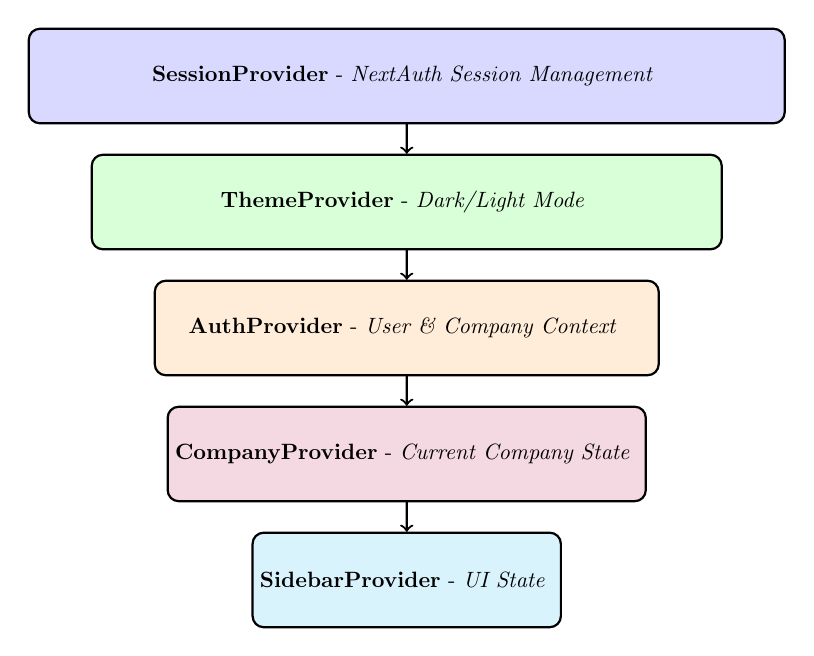
\begin{tikzpicture}[scale=0.8, every node/.style={transform shape}]
    % Providers hierarchy
    \node[draw, rounded corners, thick, fill=blue!15, minimum width=12cm, minimum height=1.5cm, align=center] (session) at (6,6) {
      \textbf{SessionProvider} - \textit{NextAuth Session Management}
    };

    \node[draw, rounded corners, thick, fill=green!15, minimum width=10cm, minimum height=1.5cm, align=center] (theme) at (6,4) {
      \textbf{ThemeProvider} - \textit{Dark/Light Mode}
    };

    \node[draw, rounded corners, thick, fill=orange!15, minimum width=8cm, minimum height=1.5cm, align=center] (auth) at (6,2) {
      \textbf{AuthProvider} - \textit{User \& Company Context}
    };

    \node[draw, rounded corners, thick, fill=purple!15, minimum width=6cm, minimum height=1.5cm, align=center] (company) at (6,0) {
      \textbf{CompanyProvider} - \textit{Current Company State}
    };

    \node[draw, rounded corners, thick, fill=cyan!15, minimum width=4cm, minimum height=1.5cm, align=center] (sidebar) at (6,-2) {
      \textbf{SidebarProvider} - \textit{UI State}
    };

    % Arrows showing hierarchy
    \draw[->, thick] (session) -- (theme);
    \draw[->, thick] (theme) -- (auth);
    \draw[->, thick] (auth) -- (company);
    \draw[->, thick] (company) -- (sidebar);
  \end{tikzpicture}
  \caption{Hierarquia de providers e contextos do frontend.}
  \label{fig:frontend-providers}
\end{figure}

Cada contexto tem responsabilidades específicas:

\begin{itemize}
  \item \textbf{SessionProvider}: Gerencia sessão NextAuth e tokens JWT
  \item \textbf{AuthProvider}: Expõe dados do usuário autenticado e empresa
  \item \textbf{CompanyProvider}: Mantém contexto da empresa atual no dashboard
  \item \textbf{ThemeProvider}: Controla tema dark/light com persistência
  \item \textbf{SidebarProvider}: Gerencia estado da interface (sidebar, mobile)
\end{itemize}

\subsection{Sistema de Autenticação e Comunicação}

A autenticação integra NextAuth com o backend NestJS através de JWT. O serviço \texttt{api.service.ts} centraliza toda comunicação HTTP:

\begin{itemize}
  \item \textbf{Token Management}: Anexa automaticamente \texttt{Bearer} tokens
  \item \textbf{Error Handling}: Trata respostas de erro padronizadas e redireciona em 401
  \item \textbf{Response Processing}: Extrai dados da estrutura padrão da API
  \item \textbf{Public Endpoints}: Diferencia rotas que não requerem autenticação
  \item \textbf{Session Validation}: Verifica validade da sessão antes de cada requisição
\end{itemize}

\subsection{Arquitetura de Componentes}

O sistema de componentes segue uma arquitetura em camadas baseada em responsabilidades:

\begin{itemize}
  \item \textbf{Primitivos UI}: Radix UI como base para acessibilidade e comportamento
  \item \textbf{Design System}: Componentes tipados (\texttt{components/ui/}) com variantes via CVA
  \item \textbf{Componentes de Domínio}: Específicos por funcionalidade (forms, tables, dialogs)
  \item \textbf{Páginas}: Composição de componentes com lógica de negócio específica
  \item \textbf{Layouts}: Estruturas reutilizáveis com providers e navegação
\end{itemize}

\subsection{Tipagem e Validação}

O TypeScript é utilizado extensivamente com tipagem específica por domínio:

\begin{itemize}
  \item \textbf{Types Directory}: Definições tipadas por entidade (\texttt{User}, \texttt{Company}, \texttt{Vehicle}, etc.)
  \item \textbf{API Responses}: Tipos padronizados para respostas da API
  \item \textbf{Form Validation}: Schemas Zod para validação client-side
  \item \textbf{Service Layer}: Métodos tipados para cada endpoint da API
  \item \textbf{NextAuth Extension}: Tipos customizados para sessão e JWT payload
\end{itemize}

Esta arquitetura garante: (i) separação clara de responsabilidades, (ii) tipagem estática end-to-end, (iii) reutilização de componentes, (iv) experiência consistente multiempresa e (v) escalabilidade via modularização por domínio.
